\newpage

\section{Auswertung}
\label{sec:Auswertung}

\subsection{Zeitkonstante des RC-Gliedes beim Entladevorgang}

Um die Zeitkonstante des Entladevorgangs des Tiefpasses zu bestimmen, wurde die Spannung $U_C(t)$ bei angelegter 
Rechteckspannung $U_S(t)$ bei einer Frequenz von 5820 Hz beobachtet. Dazu wurde ein Foto aufgenommen:

\begin{figure}
  \centering
  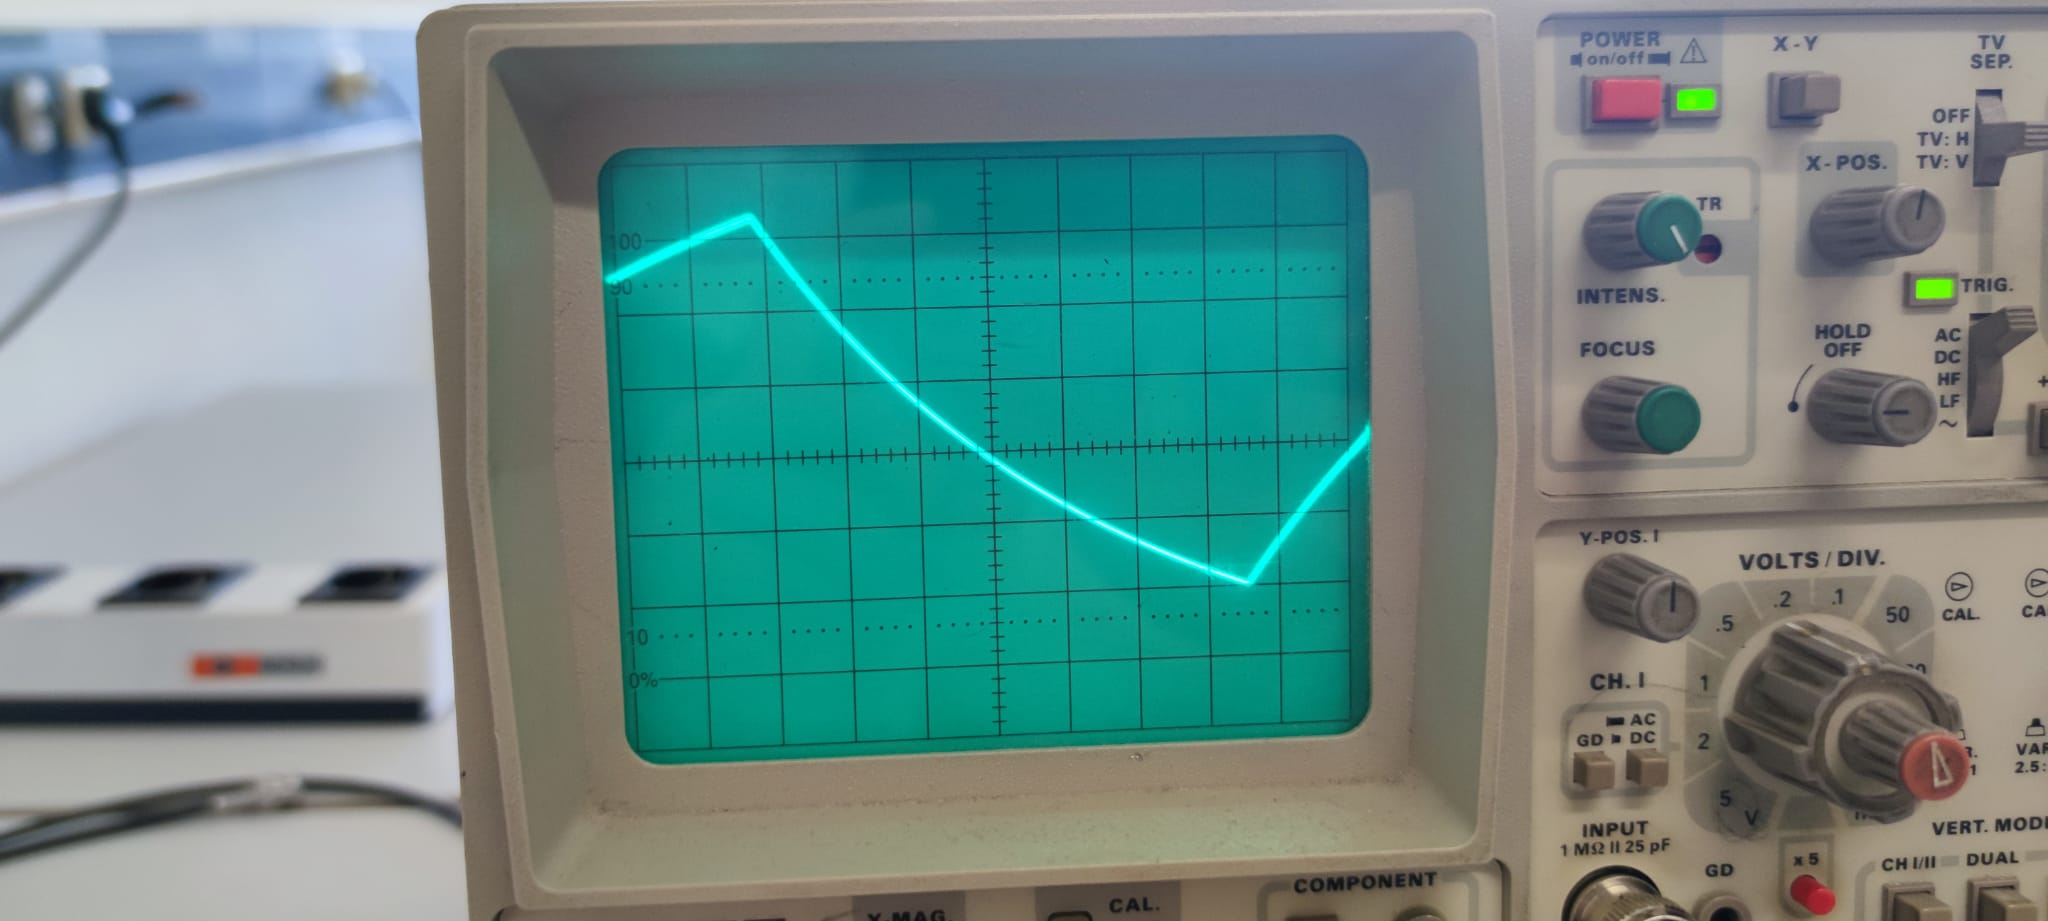
\includegraphics[width=100mm,scale=0.5]{AufgabeA.jpeg}
  \caption{Entladenvorgang des RC-Gliedes bei angelegter Rechteckspannung}
  \label{fig:AufgabeA}
\end{figure}

Der Momentaufnahme wurden fünfzehn Wertepaare entnommen, die sich in \autoref{tab:Uc,ln,T} finden lassen. Die Spannungsamplitude
wurde zu $U_0 = 1{,}1446 \, \unit{\volt}$ abgelesen.

\begin{table}
  \centering
  \caption{Ablesen von $U_{C}(t)$ zu bestimmten $t$}
  \label{tab:Uc,ln,T}
  \begin{tabular}{c c c}
    \toprule
    $U_C(t)/\unit{\volt}$ & $\ln{\left(\frac{U_C}{U_0}\right)}$ & $t/\mu \unit{\second}$ \\
    \midrule
    1.0974   &   -0.042111   &   1   \\
    0.9912   &   -0.143894   &   2.5  \\
    0.885    &   -0.257223   &   5   \\
    0.767    &   -0.400324   &   7.5  \\
    0.6608   &   -0.549359   &   10    \\
    0.5546   &   -0.724563   &   12.5  \\
    0.4838   &   -0.861139   &   15   \\
    0.413    &   -1,01936    &   17.5  \\
    0.354    &   -1.17351    &   20    \\
    0.2832   &   -1.39666    &   22.5  \\
    0.2242   &   -1.63027    &   25   \\
    0.1888   &   -1.80212    &   27.5  \\
    0.1416   &   -2.0898     &   30    \\
    0.0944   &   -2.49527    &   32.5  \\
    0.0708   &   -2.78295    &   34   \\
    \bottomrule
  \end{tabular}
\end{table}

Mit der \autoref{eqn:Entladung} lässt sich eine Ausgleichsrechnung für die Zeitkonstante $RC$ bestimmen:
\begin{align*}
  U_C(t)=U_0e^{-\frac{t}{RC}} + k \\
  \Leftrightarrow \ln{\left(\frac{U_C}{U_0}\right)} = -\frac{1}{RC}\cdot t + \ln{\left(\frac{k}{U_0}\right)}
\end{align*}

Das wird nun in \autoref{fig:plot1} geplotted und mit Python die Parameter ausgerechnet.

\begin{figure}
  \centering
  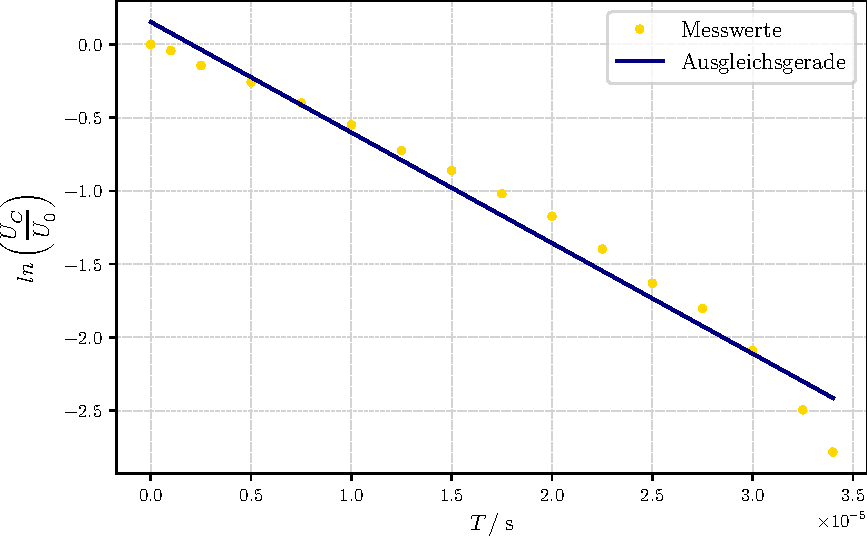
\includegraphics[width=100mm,scale=0.5]{build/plot1.pdf}
  \caption{Lineare Regression um die Zeitkonstante zu bestimmen}
  \label{fig:plot1}
\end{figure}

Damit ergibt sich für den Parameter $\ln{\left(\frac{k}{U_0}\right)}=0{,}153 \pm 0{,}071$ und für unsere Zeitkonstante $RC = (1{,}3245 \pm 0{,}0063) \, \cdot \, 10^{-5} \, \unit{\second}$.

\subsection{Ampltitude der Kondensatorspannung in Abhängigkeit von der Frequenz}

Bei dem nächsten Versuchsteil wurde die Kondensatorspannungsampltitude $A_C$ und die Speisespannungsamplitude $A_S$ in Abhängigkeit von der 
Frequenz gemessen. Es ist zu erwarten, dass die Speisespannungsamplitude nicht varriiert. Dies würde auf einen Fehler des Versuchsaufbaus hindeuten.
Es wurden die Amplituden in einem Frequenzbereich von 250 Hz bis 60 kHz gemessen, verwendet wurde diesmal eine Sinusspannung. \\
In der nachfolgenden \autoref{tab:Amplitude} wurden die Versuchsergebnisse notiert.

\begin{table}
  \centering
  \caption{Kondensatorspannungsampltituden in Abhängigkeit der Frequenz}
  \label{tab:Amplitude}
  \begin{tabular}{c c c c}
    \toprule
    $f/\unit{\hertz}$ & $A_C/\unit{\volt}$ & $A_S/\unit{\volt}$ & $\frac{A_C(\omega)}{U_0}$ \\
    \midrule      
    250    &   3.90  &   1.60  & 2.44 \\      
    500    &   3.90  &   1.60  & 2.44  \\    
   1000    &   3.60  &   1.60  & 2.25   \\   
   2500    &   2.90  &   1.60  & 1.81     \\ 
   5000    &   1.75  &   1.60  & 1.09      \\
   7500    &   1.25  &   1.60  & 0.78      \\
   10000    &   1.00  &   1.60 & 0.63       \\
   15000    &   0.64  &   1.60 & 0.40      \\
   20000    &   0.50  &   1.60 & 0.31       \\
   30000    &   0.34  &   1.60 & 0.21       \\
   40000    &   0.25  &   1.60 & 0.16       \\
   50000    &   0.20  &   1.60 & 0.13       \\
   60000    &   0.17  &   1.60 & 0.11       \\
    \bottomrule
  \end{tabular}
\end{table}

Mit \autoref{eqn:Amplitude} ergibt sich die Ausgleichsrechnung:
\begin{align*}
  A(\omega) = \frac{U_0}{\sqrt{1+\omega^2 R^2 C^2}} \\
  \Leftrightarrow \frac{A(\omega)}{U_0} = \frac{1}{\sqrt{1+\omega^2 R^2 C^2}}
\end{align*}

Die Formel mit den Messergebnissen wird nun in \autoref{fig:plot2} geplottet.

\begin{figure}
  \centering
  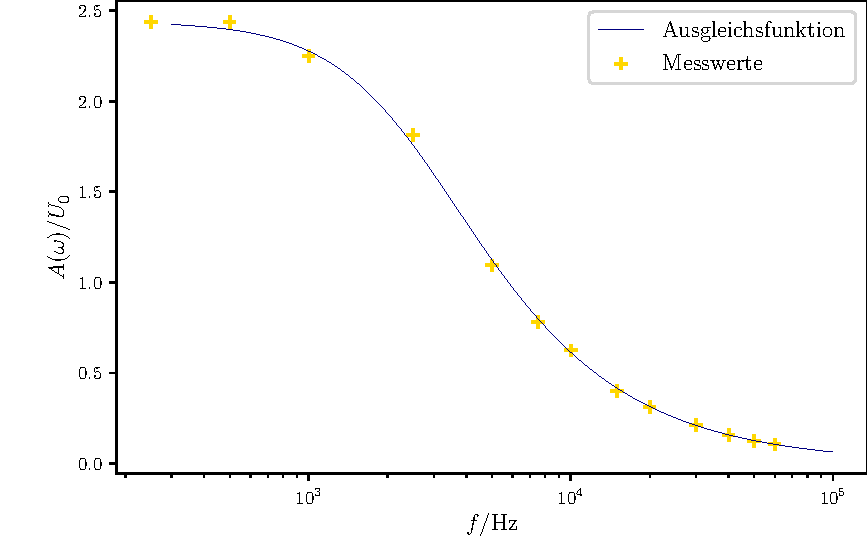
\includegraphics[width=100mm,scale=0.5]{build/plot2.pdf}
  \caption{Frequenzabhängiges Amplitudenverhätnis um die Zeitkonstante zu bestimmen}
  \label{fig:plot2}
\end{figure}

Eine lineare Ausgleichsrechnung ergibt nun $RC = (6,12 \pm 0,9) \, \cdot \, 10^{-5} \, \unit{\second}$. Die Messungenauigkeit wurde mittels
Python ermittelt.

\subsection{Phasenverschiebung des RC-Kreis}

In diesem Versuchsteil wird die Phasenverschiebung einer externen Sinusspannung und Kondensatorspannung in Abhängigkeit von der Frequenz untersucht. 
Um die Phasenverschiebung zu bestimmen, wird \autoref{eqn:phi} verwendet. Die Messwerte zu diesem Versuch lassen sich in \autoref{tab:ab} finden.

\begin{table}
  \centering
  \caption{Messwerte von a und b in Abhängigkeit der Frequenz}
  \label{tab:ab}
  \begin{tabular}{c c c c}
    \toprule
    $f/\unit{\hertz}$ & $a/\unit{\second}$ & $b/\unit{\second}$ & $\varphi / rad$ \\
    \midrule      
      250 & 0.000025 & 0.001500 & 0.104720 \\
      500  &0.000025 & 0.001500 & 0.104720\\
      1000 & 0.000022&  0.000390 & 0.354436\\
      2500 & 0.000019 & 0.000170&  0.702238\\
      5000&  0.000012 & 0.000078&  0.966644\\
      7500 & 0.000010 & 0.000052 & 1.208305\\
      10000 & 0.000008 & 0.000039&  1.288859\\
      15000 & 0.000006 & 0.000026 & 1.449966\\
      20000 & 0.000005 & 0.000020 & 1.413717\\
      30000 & 0.000003 & 0.000013 & 1.449966\\
      40000 & 0.000002  &0.000010 & 1.507964\\
      50000&  0.000002 & 0.000008 & 1.570796\\
      60000 & 0.000002 & 0.000006 & 1.675516\\
    \bottomrule
  \end{tabular}
\end{table}

Mit den Messwerten, wurde mittels Python $\varphi$ gegen die Frequenz geplotted, woraus die Zeitkonstante $RC$ bestimmt wird: $RC = (5,37 \pm 0,00002) \, \cdot \, 10^{-5} \, \unit{\second}$.

\begin{figure}
  \centering
  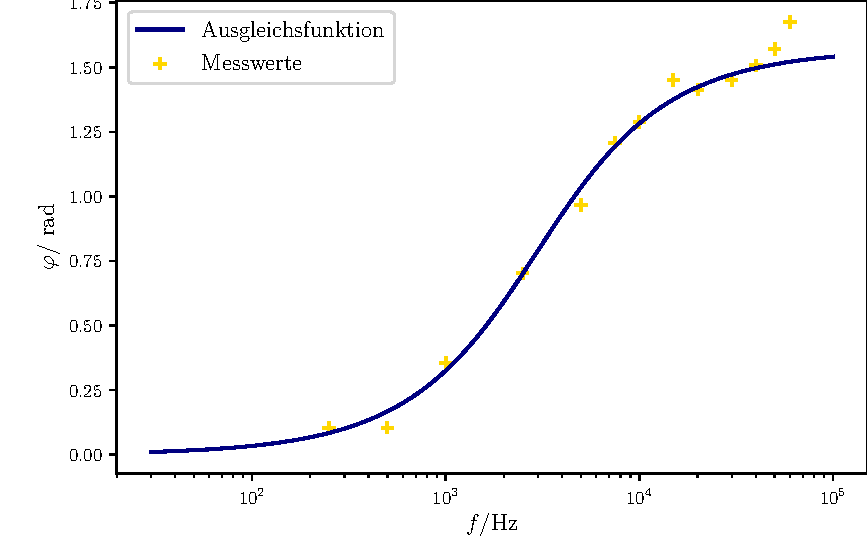
\includegraphics[width=100mm,scale=0.5]{build/plot3.pdf}
  \caption{Phasenverschiebung}
  \label{fig:plot3}
\end{figure}

\subsection{RC-Kreis als Integrator}

Mithilfe der Ergebnisse der Phasenverschiebung und unseren Messwerte aus dem Versuchsteil davor, lässt sich eine neue Tabelle aufstellen. In dieser Tabelle
wird die Phasenverschiebung mit dem Amplitudenverhältnis verglichen.

\begin{table}
  \centering
  \caption{Amplitudenverhältnis und Phasenverschiebung}
  \label{tab:Uphi}
  \begin{tabular}{c c}
    \toprule
    $U_C/\unit{\volt}$ & $\varphi / rad$ \\
    \midrule      
    2.44  & 0.104720 \\
    2.44  & 0.104720\\
    2.25  & 0.354436\\
    1.81  &  0.702238\\
    1.09  &  0.966644\\
    0.78  & 1.208305\\
    0.63  &  1.288859\\
    0.40  & 1.449966\\
    0.31  & 1.413717\\
    0.21  & 1.449966\\
    0.16  & 1.507964\\
    0.13  & 1.570796\\
    0.11  & 1.675516\\
    \bottomrule
  \end{tabular}
\end{table}

Zu diesen Wertepaaren ist nun eine alternative Darstellung mittels eines Polarplots möglich. Dieser ist in \autoref{Abb:Polar} zu sehen.
\begin{figure}
  \centering
  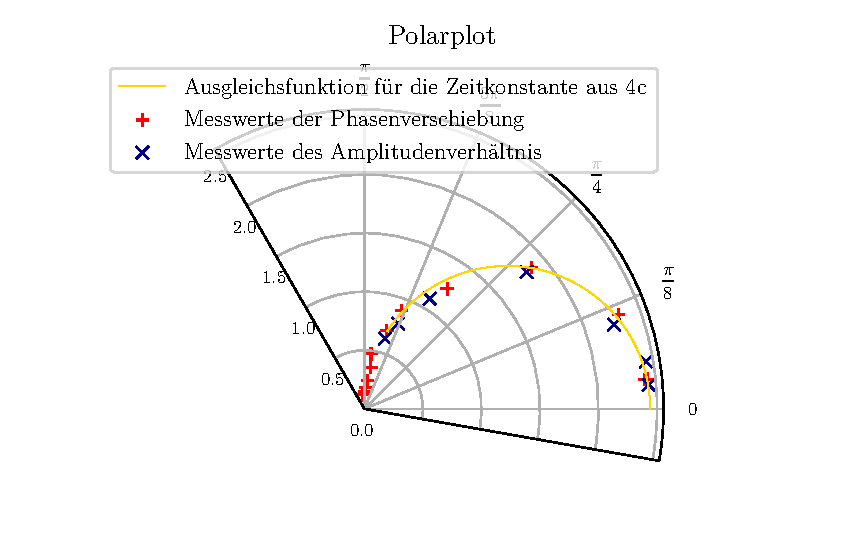
\includegraphics[width=100mm,scale=0.5]{build/polarplot.pdf}
  \caption{Polarplot}
  \label{Abb:Polar}
\end{figure}

Radial ist das Amplitudenverhältnis abzulesen und in dem Polarwinkel die Phasenverschiebung. Da der Erwartungswert mit dem Realwert
des Oszilloskops übereinstimmt, ist die Integrierbarkeit des RC-Kreises bewiesen. \\
Zur weiteren Untersuchung der Integrator-Identität des RC-Kreises wurden in \autoref{Spannungen} drei verschiedene Wechselspannungen angelegt:
\begin{figure}
	\centering
	\begin{subfigure}[b]{0.3\textwidth}
		\centering
		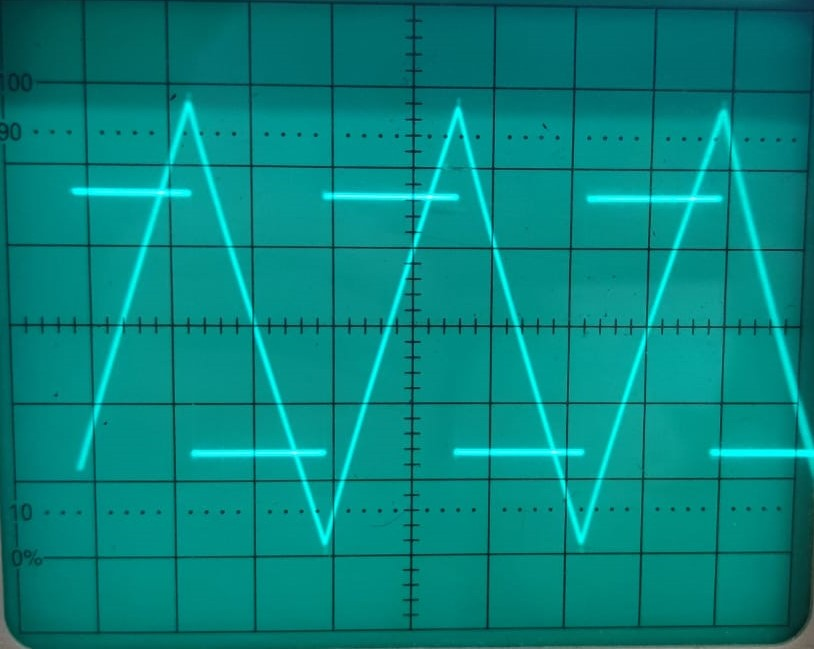
\includegraphics[width=4.5cm]{build/integrator-rechteck.jpeg}
		\caption{Rechteckschwingung}
	\end{subfigure}
	~
	\begin{subfigure}[b]{0.3\textwidth}
		\centering
		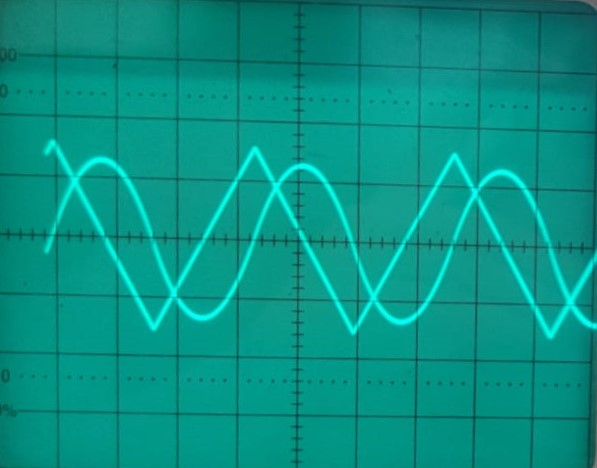
\includegraphics[width=4.5cm]{build/integrator-saegezahn.jpeg}
		\caption{Dreieckschwingung}
	\end{subfigure}
	~
	\begin{subfigure}[b]{0.3\textwidth}
		\centering
		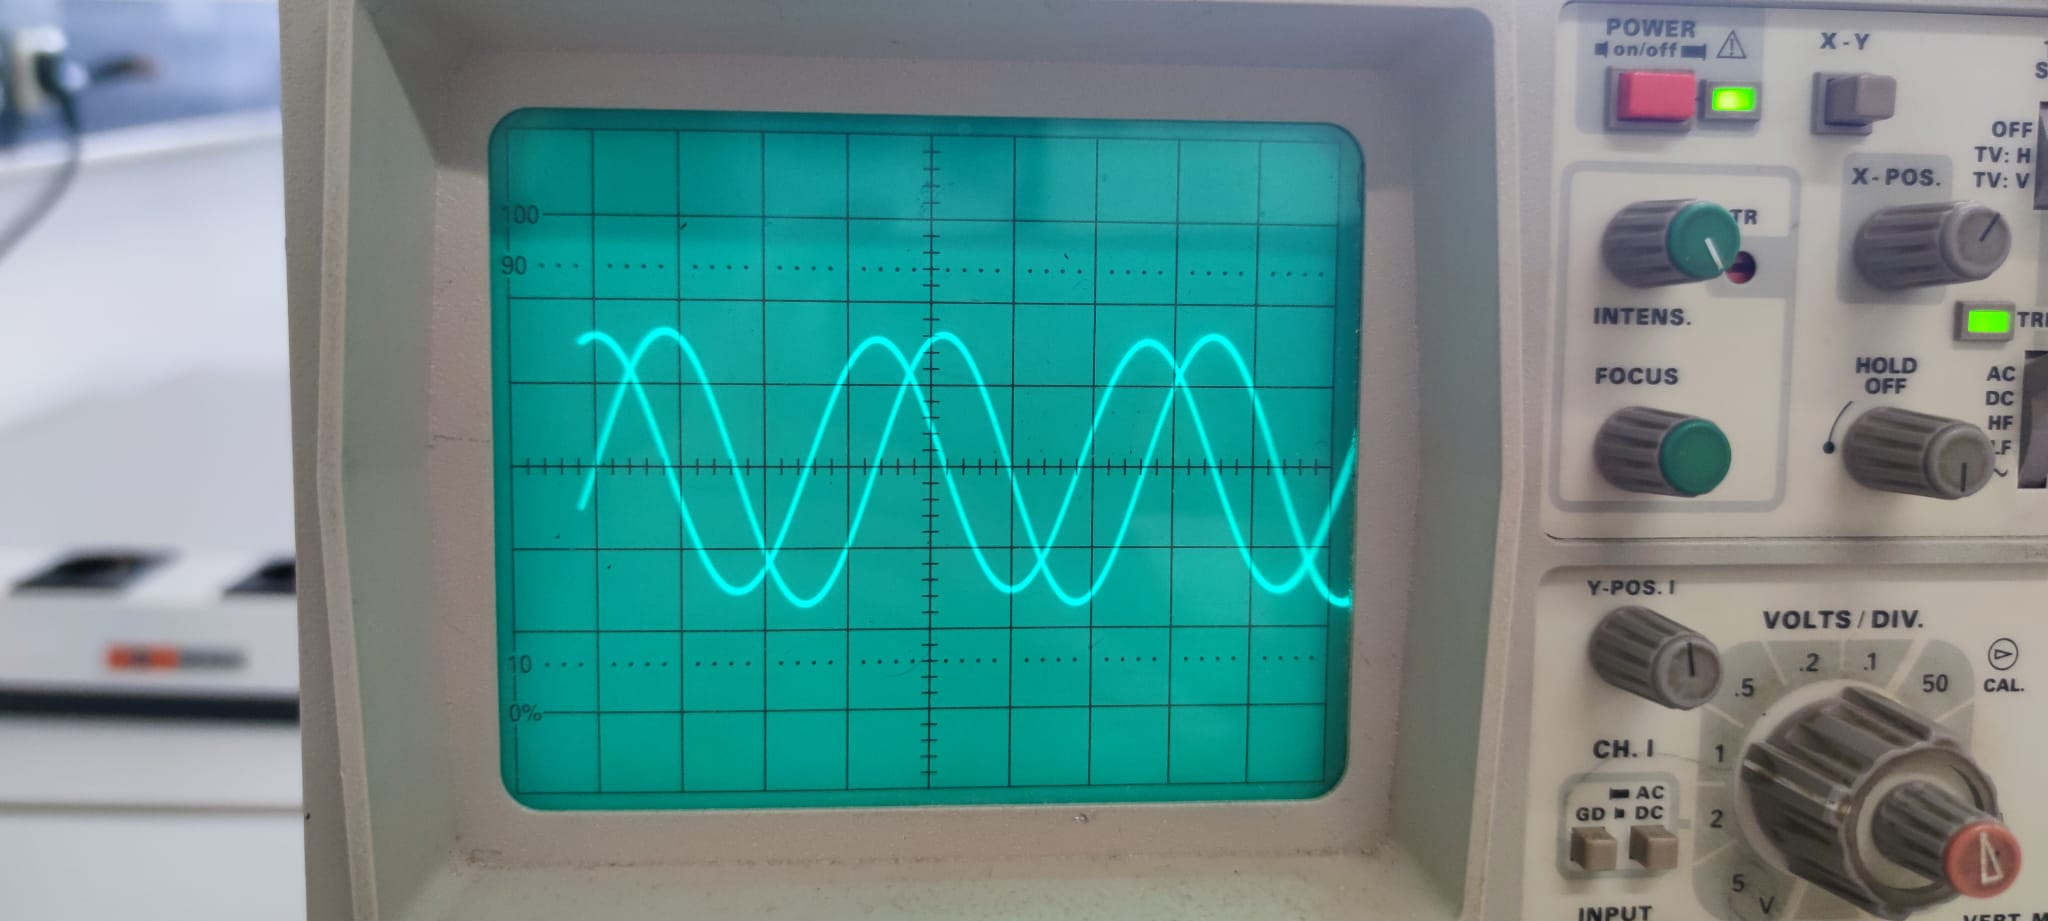
\includegraphics[width=4.5cm]{build/integrator-sinus.jpeg}
		\caption{Sinus-Schwingung}
	\end{subfigure}
  \caption{Drei verschiedene Spannungen}
  \label{Spannungen}
\end{figure}

